%%
%% ****** ljmsamp.tex 13.06.2018 ******
%%
\documentclass[
11pt,%
tightenlines,%
twoside,%
onecolumn,%
nofloats,%
nobibnotes,%
nofootinbib,%
superscriptaddress,%
noshowpacs,%
centertags]%
{revtex4}
\usepackage{ljm}
\usepackage{listings}
\usepackage{amsmath,amsthm,amscd,amsfonts,amssymb}
\usepackage{textcomp}
\usepackage{graphicx}
\usepackage{esvect}
\usepackage{physics}

\lstset{
language=C++,
basewidth=0.5em,
xleftmargin=45pt,
xrightmargin=45pt,
basicstyle=\small\ttfamily,
keywordstyle=\bfseries\underbar,
numbers=left,
numberstyle=\tiny,
stepnumber=1,
numbersep=10pt,
showspaces=false,
showstringspaces=false,
showtabs=false,
frame=trBL,
tabsize=2,
captionpos=t,
breaklines=true,
breakatwhitespace=false,
escapeinside={\%*}{*)}
}

\begin{document}

\titlerunning{Deformation of the surface mesh in the two-dimensional case} % for running heads
\authorrunning{A.~A.~Rybakov and S.~S.~Shumilin} % for running heads
%\authorrunning{First-Author, Second-Author} % for running heads

\title{Approximate methods of deformation of the surface mesh in the two-dimensional case}
% Splitting into lines is performed by the command \\
% The title is written in accordance with the rules of capitalization.

\author{\firstname{A.~A.}~\surname{Rybakov}}
\email[E-mail: ]{rybakov.aax@gmail.com} \affiliation{Joint
Supercomputer Center of the Russian Academy of Sciences (JSCC RAS)
-- Branch of Scientific Research Institute of System Analysis of the
Russian Academy of Sciences, Leninsky prospect 32a, Moscow, 119334,
Russia}

\author{\firstname{S.~S.}~\surname{Shumilin}}
\email[E-mail: ]{shumilin@jscc.ru} \affiliation{Joint Supercomputer
Center of the Russian Academy of Sciences (JSCC RAS) -- Branch of
Scientific Research Institute of System Analysis of the Russian
Academy of Sciences, Leninsky prospect 32a, Moscow, 119334, Russia}
%\noaffiliation % If the author does not specify a place of work.

\firstcollaboration{(Submitted by TODO : SUBMITTER)} % Add if you know submitter.
%\lastcollaboration{ }

\received{TODO : DATE} % The date of receipt to the editor, i.e. December 06, 2017

\begin{abstract}
Numerical simulation of the surface ice accretion includes the work of various solvers that are performed iteratively and exchange data with each other.
The calculation execution chain consists of the work of the gas-dynamic solver, the calculation of the liquid phase, the calculation of the thickness of the accreted ice on the surface grid and the rebuilding of the surface.
After rebuilding is done, the modelling process goes to the next iteration in the gas-dynamic solver.
Thus, the performance of a qualitative rebuilding of the surface computational grid taking into account the accumulated ice affects all further calculations.
The article discusses approximate methods of rebuilding the surface mesh according to the ice accretion in each cell for the two-dimensional case and estimates their accuracy.
\end{abstract}

\subclass{TODO : CODE} % Enter 2010 Mathematics Subject Classification.

\keywords{Mesh deformation, displaced areas, gradient descend} % Include keywords separeted by comma.

\maketitle

% Text of article starts here.

\section{Introduction}

The task of calculating the ice accretion of aerodynamic surfaces is extremely relevant today.
Of the most well-known software products that implement this functionality, we can emphasize such packages as FENSAP-ICE \cite{Bourgault_FENSAP}, LEWICE \cite{Bidwell_LEWICE}, CANICE \cite{Pueyo_CANICE}, CHT2D \cite{Pueyo_CHT2D} and many others.
As a rule, these packages are multi-step and provide for iterative rebuilding of the surface mesh as the ice increases.
Such rebuilding is required to be performed, as with the growth of ice, it is necessary to re-launch the aerodynamic solver to obtain actual data on the motion of the medium around the new deformed body. \cite{Ozgen, Beaugendre}.
To obtain a more accurate profile of accreted ice, it is required to rebuild the surface mesh as often as possible, therefore, the speed of the mesh rebuilding algorithms is also significant.

Of particular interest is the development of algorithms for rebuilding surface grids in three-dimensional space.
Among them there is a rebuilding algorithm with local saving of the cell volume \cite{Jiao}, which found its implementation in the iceSurf tool \cite{Thompson}.
However, work on the development of algorithms for rebuilding surfaces in two-dimensional space is also under way, and the results of these studies are more-less transferred to work in three-dimensional space, as demonstrated in \cite{Pueyo}.

In this paper, we have analyzed approximate methods for rebuilding a surface mesh only for the two-dimensional case; however, they can be generalized to three-dimensional objects.
Further, the task of rebuilding the surface mesh is considered in an abstract form without reference to the problems of ice accretion.

\section{Problem of rebuilding the surface in two-dimensional space}

Consider the geometric problem of rebuilding a surface in two-dimensional space in general form.
Let $n$ cells of the surface grid be given, each of which is represented by a segment of length $l_i$ (that is, the total number of nodes is $n+1$).
The direction of change of the surface of each cell is known (the direction of the normal to the segment), as well as the direction of movement of each node $\overline{g_i}$, $|\overline{g_i}| = 1$.
It coincides with the direction of the sum of the unit normals drawn to the incident cells.
Moreover, for a two-dimensional case, this direction lies on the bisector of the angle formed by two incident cells \cite{Fortin} (Fig.~\ref{fig:grid_normals}).

\begin{figure}[h]
\setcaptionmargin{5mm}
\onelinecaptionstrue
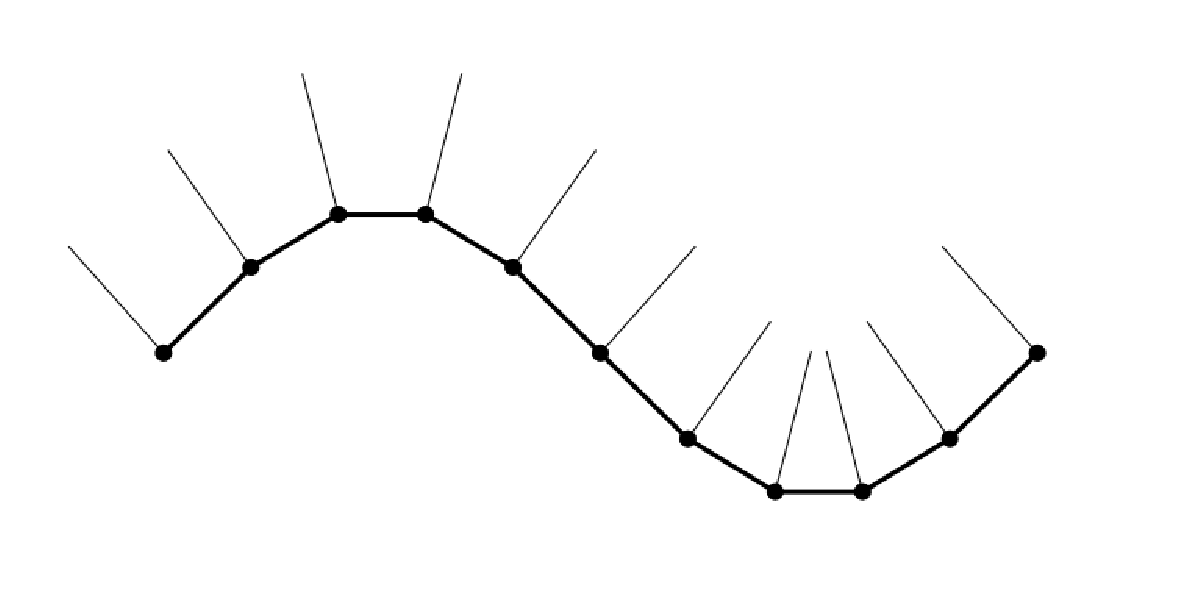
\includegraphics[width=0.8\textwidth]{pics/grid_normals.pdf}
\captionstyle{normal}\caption{Surface mesh with designated direction of movement of the nodes.}
\label{fig:grid_normals}
\end{figure}

It is required to find such values of local shifts of grid nodes $h_i$ that the covering area between the old surface and the new surface for each grid cell ($S_i$) differ as small as possible from the required value a $T_i = l_iH_i$.

To solve this problem, first, it's needed to calculate the covering area for each individual cell.

\subsection{The task of calculating the covering area when moving nodes of a single cell}

Consider a cell represented on a plane by a segment $AB$ of length $l$.
When moving $A$ and $B$ to the new points $A_1$ and $B_1$ respectively quadrangle $AA_1B_1B$ is formed.
It is required to find its area expressed explicitly through parameters $a = \overline{AA_1}$ и $b = \overline{BB_1}$ (Fig.~\ref{fig:local}).

\begin{figure}[h]
\setcaptionmargin{5mm}
\onelinecaptionstrue
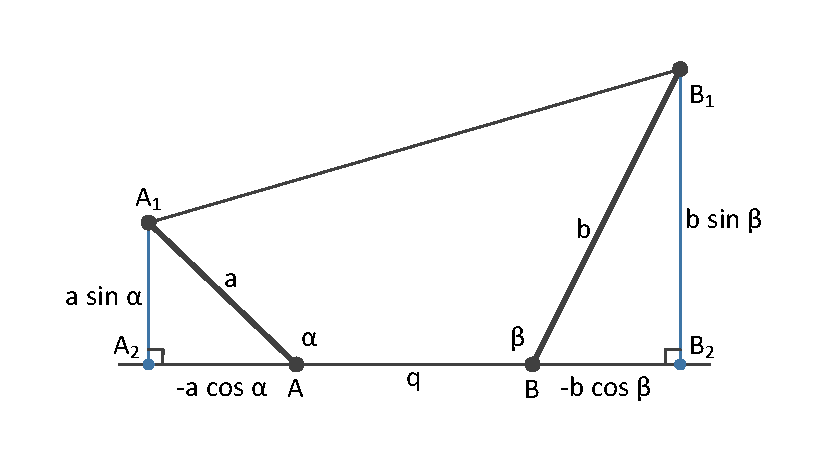
\includegraphics[width=0.8\textwidth]{pics/local.pdf}
\captionstyle{normal}\caption{Calculation of the covering area when moving the nodes of the cell.}
\label{fig:local}
\end{figure}

To solve the problem, we drop perpendiculars from the points $A_1$ and $B_1$ to a straight $AB$.
Their projections will be points $A_2$ and $B_2$ respectively.
The required area can be represented as follows:

\begin{equation}
S_{AA_1B_1B} = S_{A_2A_1B_1B_2} - S_{AA_1A_2} - S_{BB_1B_2}
\end{equation}

Denote the angle between the vectors $\overline{AA_1}$ and $\overline{AB}$ as $\alpha$, and the angle between the vectors $\overline{BB_1}$ and $\overline{BA}$ as $\beta$.
Then the required area is calculated explicitly in the following form:

\begin{equation}
S_{AA_1B_1B} = \frac{1}{2}(l - a \cos \alpha - b \cos \beta)(a \sin \alpha + b \sin \beta) + \frac{1}{2}a^2 \sin \alpha \cos \alpha + \frac{1}{2}b^2 \sin \beta \cos \beta
\end{equation}

\begin{equation}
S_{AA_1B_1B} = \frac{1}{2}\big(l(a \sin \alpha + b \sin \beta) - ab \sin(\alpha + \beta)\big)
\end{equation}

\subsection{Gradient Descent Solution}

The gradient descent method is one of the simplest optimization method for finding the local minimum of a function.
Provided that at any point of the function it is possible to calculate its gradient, then an iteration sequence is constructed starting from some initial approximation $x_0$.~\cite{Kantorovich}:

\begin{equation}
x^{k+1} = x^k - \gamma _k \nabla f(x_k)
\end{equation}

where $\gamma _k \geq 0$ sets the step length and, respectively, the rate of gradient descend.

The gradient method finds its main application in the task of finding the minimum or maximum of a function.
The direction of the anti-gradient is the direction of the fastest decreasing of the function.
The main problem of the method is to choose the step $\gamma$.
For large values of the step, there is a chance to "jump over" the minimum of the function.
In addition, the method does not guarantee finding a global minimum.

Consider the solution of the problem by the method of gradient descent.
The unknown parameters are the magnitudes of the shifts of the nodes of the grid $h_i$.
Based on the solution of the local problem of determining the covering area, we can define the covering area when a separate cell moves as:

\begin{equation}
S_i = \frac{1}{2}\big(l_i(h_i \sin \alpha_i + h_{i + 1} \sin \beta_i) - h_ih_{i + 1} \sin(\alpha_i + \beta_i)\big) 
\end{equation}

The deviation of the covering area in the cell from the true value will be called the value $\delta_i = S_i - T_i$, and its error is its square $d_i = \delta_i^2$.
The total error when rebuilding the surface is defined as the sum of errors for all cells:

\begin{equation}
D = \sum_{i = 0}^{n - 1}{d_i}
\end{equation}

When finding the optimal solution, it is required to minimize the total error.
To find the gradient, it is required to calculate the partial derivatives of the function $D$ over all unknowns $h_i$.
These derivatives can be written explicitly.

\begin{equation}
\frac{\partial D}{\partial h_i} = \frac{\partial d_{i - 1}}{\partial h_i} + \frac{\partial d_i}{\partial h_i}
\end{equation}

where

\begin{equation}
\begin{cases}
\frac{\partial d_{i - 1}}{\partial h_i} = \delta_{i - 1}(l_{i - 1} \sin \beta_{i - 1} - h_{i - 1} \sin(\alpha_{i - 1} + \beta_{i - 1})) \\
\frac{\partial d_i}{\partial h_i} = \delta_i(l_i \sin \alpha_i - h_{i + 1} \sin(\alpha_i + \beta_i))
\end{cases}
\end{equation}

Also, when implementing the gradient descent method, it is required to monitor the compliance of additional conditions that are imposed on the unknown $h_i$.
For example, an obvious condition is that $h_i \ge 0$ is satisfied, which prevents the grid from moving in a negative direction.
In this work, more stringent conditions $min(H_{i - 1}, H_i) \le h_i \le max(H_{i - 1}, H_i)$ were used, which do not allow the values of the displacement of the grid nodes to go beyond the limits of the displacements of the grid cells incident to them.

\section{Approximate solution schemes}

Solving the problem of rebuilding the grid using the gradient descent method is too resource-demanding as the grid size increases.
In addition, the quality of the solution is often unsatisfactory, especially when hit in local minima.
Therefore, to solve the problem, methods of approximate solution were proposed, based on approximation of the solution in each cell using primitive geometric shapes.

\subsection{Solution by rectangles method}

As a first method, we consider an approximation in which each grid node is shifted by a vector $\frac{1}{2}(H_{i - 1} + H_i)\overline{g_i}$.
This method corresponds to the approximation of the solution in each cell with a rectangle on the sides of $l_i$ and $H_i$, and then averaging, as shown in Fig.~\ref{fig:grid_rectangles}.

\begin{figure}[h]
\setcaptionmargin{5mm}
\onelinecaptionstrue
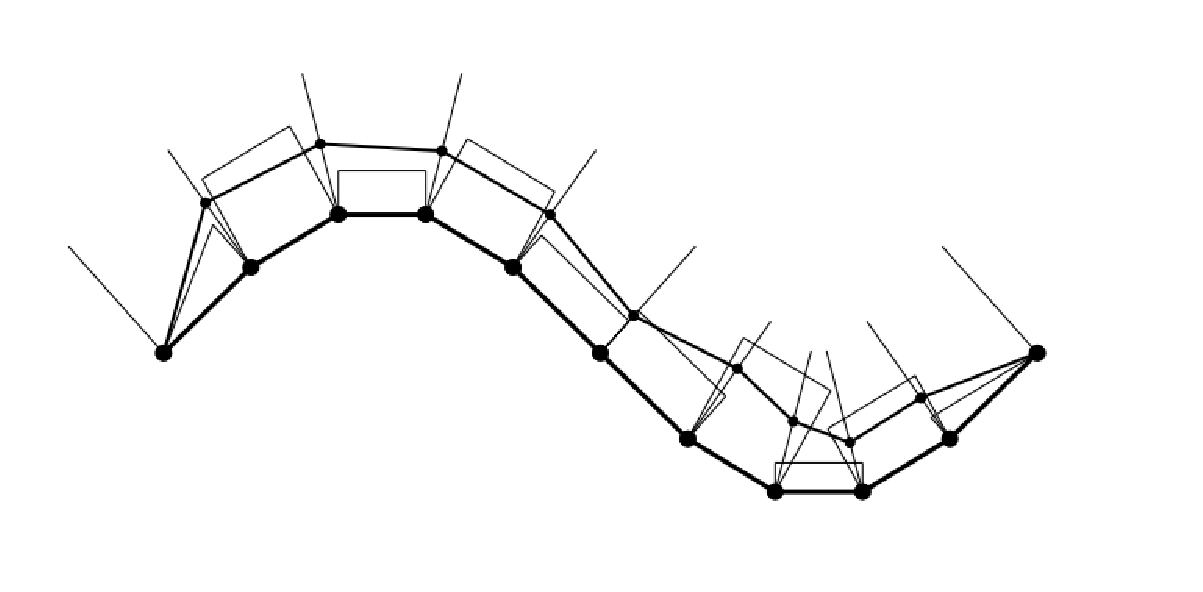
\includegraphics[width=0.8\textwidth]{pics/grid_rectangles.pdf}
\captionstyle{normal}\caption{Surface rebuilding using the rectangle method.}
\label{fig:grid_rectangles}
\end{figure}

It is worth noting the possible development of this approach through the use of multilayer approximation, as described in \cite{Bourgault_Cote}, however, this opportunity was not considered in this paper.

\subsection{Solution by trapezoid method}

In the trapezoid method, the solution in each cell is approached by a trapezoid with an area of $T_i$, the sides of which lie on the growth directions of two nodes belonging to the considered cell.
After constructing the trapezoid for all grid cells, each internal node has two new potential positions for the shift (formed by the cell on the left and the cell on the right).
Their average value is chosen as the final position. (Fig.~\ref{fig:grid_trapeziums}).

\begin{figure}[h]
\setcaptionmargin{5mm}
\onelinecaptionstrue
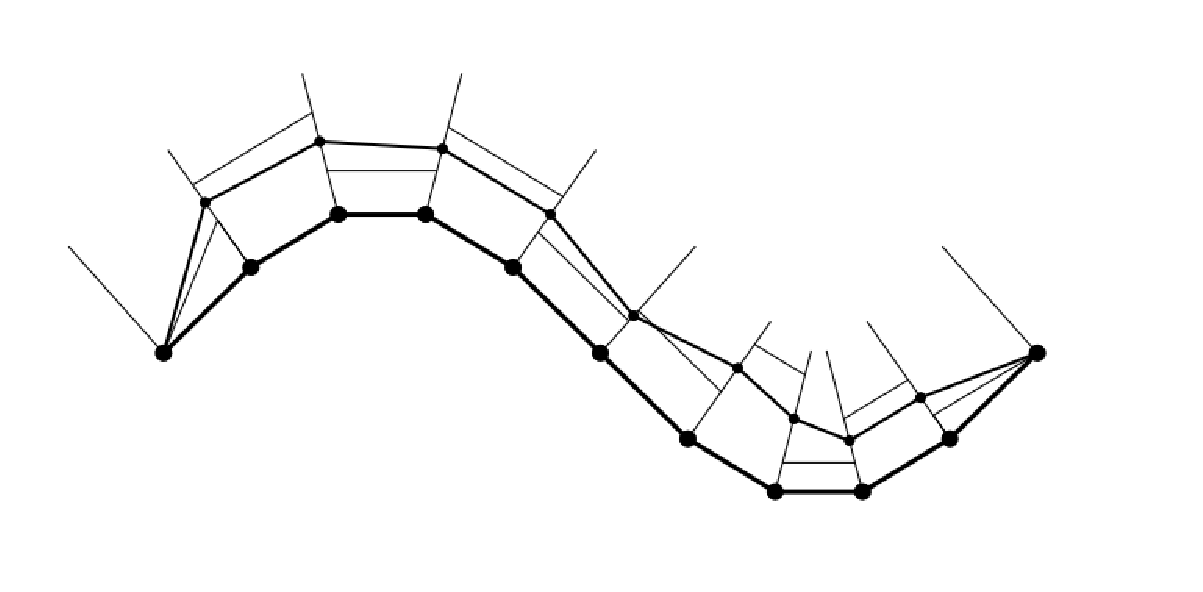
\includegraphics[width=0.8\textwidth]{pics/grid_trapeziums.pdf}
\captionstyle{normal}\caption{Surface rebuilding by trapezoid method.}
\label{fig:grid_trapeziums}
\end{figure}

\subsection{Comparison of solution accuracy}

To compare the accuracy of the solutions obtained using the methods described, we used a model two-dimensional surface grid represented by a single sinusoid period ($x \in [0, 2 \pi]$).
As a set of cell shifts ($ H_i $), the same shifts equal to half of cell size were used.
With an increase in the number of nodes, both approximate methods demonstrated values $\frac{D}{\sum_i{T_i}}$ tending to zero with minor deviations from each other and from the gradient descent method that was used for verification.
A comparison of the values of $\delta_i$ for all cells for the proposed approximate methods was also carried out.
The results of the comparison on the model grid with the number of nodes $n = 1000$ are shown Fig.~\ref{fig:graphic}.

\begin{figure}[h]
\setcaptionmargin{5mm}
\onelinecaptionstrue
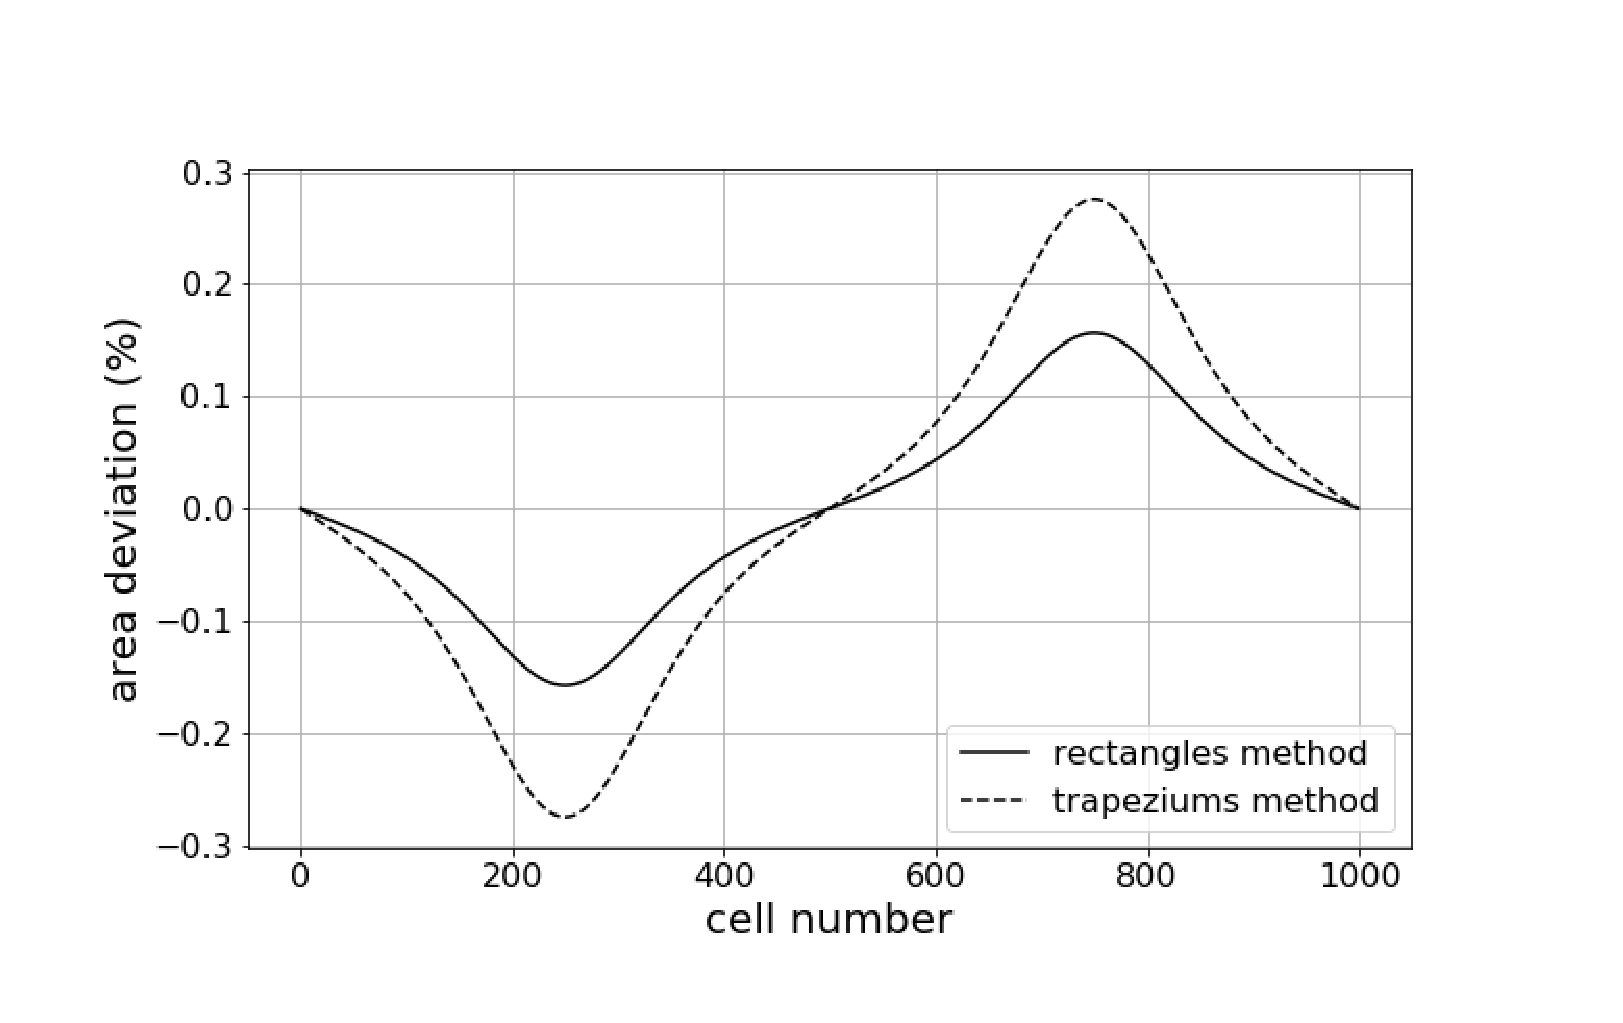
\includegraphics[width=1.0\textwidth]{pics/graphic.pdf}
\captionstyle{normal}\caption{Comparison of the accuracy of solutions using the rectangle method and the trapezoid method.}
\label{fig:graphic}
\end{figure}

It can be seen from this graph that the simpler method of rectangles is at the same time more accurate, since it provides smaller deviations from the exact solution on strongly convex and strongly concave sections of the grid.

\section{Conclusion}

Two simple approximate methods for rebuilding a surface mesh in two-dimensional space were considered.
Comparison of the results of their work with a locally optimal solution obtained using the iterative gradient descent method showed the inexpediency of using the latter for industrial calculations.
Of the two approximate rebuilding methods, the rectangle method demonstrated smaller deviations of the solution for individual grid cells in places of strong grid curvature.
The considered approximate methods can be extended to the three-dimensional case, but this is beyond the scope of this article.

\begin{acknowledgments}
The work was done at the JSCC RAS as part of the state assignment for the topic 0065-2019-0016 (reg. no. AAAA-A19-119011590098-8). The supercomputer MVS-10P, located at the JSCC RAS, was used for calculations during the research.
\end{acknowledgments}

\begin{thebibliography}{99}

\bibitem{Bourgault_FENSAP}
\refitem{article}
Y.~Bourgault, H.~Beaugendre, W.~G.~Habashi, {\it ``Development of a shallow-water icing model in FENSAP-ICE"}, Journal of Aircraft, Vol.~37, No.~4, 640 -- 646 (2000).

\bibitem{Bidwell_LEWICE}
\refitem{article}
C.~Bidwell, D.~Pinella, P.~Garrison, {\it ``Ice accretion calculations for a commercial transport using the LEWICE3D, ICEGRID3D and CMARC programs"}, AIAA Paper 99-0250, Reno (1999).

\bibitem{Pueyo_CANICE}
\refitem{articlce}
A.~Pueyo, D.~Chocron, F.~Kafyeke, {\it ``Improvements to the ice accretion code CANICE"}, CASI $8^{TH}$ Aerodynamics Symposium, Toronto (2001).

\bibitem{Pueyo_CHT2D}
\refitem{article}
A.~Pueyo, D.~Chocron, F.~Mokhtarian, F.~Kafyeke, {\it ``CHT2D: A 2D hot air anti-icing analysis tool"}, $50^{TH}$ Annual General Meeting (AGM) and Conference, Canadian Aeronautics and Space Institute (2003).

\bibitem{Ozgen}
\refitem{article}
S.~\"Ozgen, M.~Canibek, {\it ``Ice accretion simulation on multi-element airfoils using extended Messinger model"}, Heat Mass Transfer, 45, 305 -- 322 (2009).

\bibitem{Beaugendre}
\refitem{article}
H.~Beaugendre, {\it ``A PDE-based 3D approach to in-flight ice accretion"}, PHD Thesis, McGill University, Montreal, QC (2003).

\bibitem{Jiao}
\refitem{article}
J.~Jiao, {\it ``Volume and feature preservation in surface mesh optimization"}, Proceedings, $15^{TH}$ International Meshing Roundtable, Springer-Verlag, Birmingham, AL, 359 -- 374 (2006).

\bibitem{Thompson}
\refitem{article}
D.~Thompson, X.~Tong, Q.~Arnoldus, E.~Collins, D.~McLaurin, E.~Luke, {\it ``Discrete surface evolution and mesh deformation for aircraft icing applications"}, In $5^{TH}$ AIAA Atmospheric and Space Environments Conference. AIAA Paper 2013-2544 (2013).

\bibitem{Pueyo}
\refitem{article}
A.~Pueyo, {\it ``Efficient 3D artificial ice shapes simulations with 2D ice accretion codes using a 3-level correction"}, In SAE 2013 AeroTech Congress and Exhibition, Vol.~7, SAE Technical Paper 2013-01-2136 (2013).

\bibitem{Fortin}
\refitem{article}
G.~Fortin, A.~Ilinca, J.-L.~Laforte, V.~Brandi, {\it ``New roughness computation method and geometric accretion model for airfoil icing"}, Journal of Aircraft, Vol.~41, No.~1, 119-127 (2004).

\bibitem{Kantorovich}
\refitem{book}
G.~P.~Akilov, L.~V.~Kantorovich, {\it ``Functional analysis"}, 2nd ed., Pergamon Press (1982). 

\bibitem{Bourgault_Cote}
\refitem{article}
S.~Bourgault-C\^ot\'e, K.~Hasanzadeh, P.~Lavoie, E.~Laurendeau, {\it ``Multi-layer icing methodologies for conservative ice growth"}, In $7^{TH}$ European Conference for Aeronautics and Aerospace Sciences (EUCASS) (2017).

\end{thebibliography}

\end{document}
